% !TEX program = xelatex
\documentclass[a4paper, 11pt, final]{article}
\usepackage{latexsym}
%\usepackage{ctex}
% 绘制三线表
\usepackage{booktabs}
% 排版图片
\usepackage{subfig}
\usepackage{graphicx}
% 数学公式
\usepackage{amsmath}
\usepackage{amssymb}
\usepackage{indentfirst}
% 格式设定
\setlength{\topmargin}{0.0cm} \setlength{\headsep}{0.0cm}
\setlength{\topskip}{1.5cm} \setlength{\oddsidemargin}{0.0cm}
\setlength{\evensidemargin}{0.0cm} \setlength{\textwidth}{16cm}
\setlength{\textheight}{24cm}\setlength{\parindent}{2em}
% 两个自定义命令
\renewcommand{\baselinestretch}{1.5}
\setcounter{page}{1}
\renewcommand{\theequation}{\thesection.\arabic{equation}}

% 正文
\begin{document}
% 阿拉伯数字排页码
\pagenumbering{arabic}
% 制作标题
\title
{Numerical Path Integration Based on Adaptive Bubble GridS
 for Nonlinear Dynamic Systems
 \footnotetext{$^{\dag}$ E-mail address: mpf@mail.nwpu.edu.cn (Pengfei Ma)} }

% 作者和通讯地址
\author{{Li Cai$^{\ a}$, Pengfei Ma$^{\ a}$$^{\dag}$ }\\
{\small \it $^{\ a}$ NPU-UoG International Cooperative Lab for Computation ${\&}$ Application in Cardiology}\\
{\small \it Northwestern Polytechnical University, }{\small \it Xi'an, Shaanxi 710129, China}\\
{Wenxian Xie$^{\ b}$, Wei Guo$^{\ b}$, Weiwei Zhang$^{\ b}$, {Yufeng Nie$^{\ b}$}}\\
{\small \it $^{\ b}$ School of Science, Northwestern Polytechnical University},
{\small \it Xi'an, Shaanxi 710129, China}\\
{Xiaoyu Luo$^{\ c}$, Hao Gao$^{\ c}$}\\
{\small \it $^{\ c}$ School of Mathematics and Statistcs, University of Glasgow, Glasgow G12 8SQ, UK}
}
\date{}
\maketitle
% reserved 下面三行还不知道什么意思
\pagestyle{myheadings} \markboth{W.X.~XIE et
al}{\footnotesize{Numerical Path Integration Based on Adaptive Bubble Grids
for Nonlinear Dynamic Systems}}
% 摘要
\begin{abstract}
    A new numerical path integration method based on adaptive bubble grids
   for nonlinear dynamic systems is proposed in this paper. 
   Bubble nodes are adjusted depending on the changing of probability density.
   For every step before path integration, grids are regenerated using adaptive bubble
   grids method. The results are better if bubble nodes gather where the
   value of probability density is large.
   Besides, GPU accelaration is used in bubble grids algorithm which makes our 
   method much more efficient. Numerical results of Duffing
   oscillator subjected to white noise exitation were calculated and compared with
   the exact stationary solutions. Finally, the transitions of probability density
   for Duffing oscillator subjected to harmonic and stochastic excitations are
   captured precisely with the method proposed in this paper.

\end{abstract}
{\bf Keywords:}\quad\/ 
path integration method, adaptive bubble grids, nonlinear dynamic systems
\maketitle
% 正文部分
\section{Introduction}
Stochastic dynamical systems can be used to model a wide variety of
practical problems in natural science and engineering applications.
Once the response of a dynamical system with Gaussian white noise
excitations is a diffusion process, then the transition probability
density of the response is governed by the Fokker-Planck-Kolmogorov
(FPK) equation \cite{ZWQ2017,GCW1986}.

Instead of solving the FPK equation directly, the path integration
method is a more natural and powerful numerical method for capturing
the evolution of the probability density. The numerical implementation
of the above technique consists in using the Chapman-Smoluchowski
equation to follow the time evolution of the process through small
elementary steps and then employing the appropriate interpolation
procedures. 

Every existing path integration procedure used a certain integration
scheme in which the probability density is represented by its values
at discrete grid points. Among the first systematic efforts to develop
the path integration method into a numerical tool were those of Wehner
et al. \cite{1}-\cite{3} , and the piecewise constant interpolation scheme used in
their papers. The interpolation by cubic B-spline function was used by
Naess et al. \cite{4} to gain a satisfactory probability density accurate
at the tails. The numerical path integration method based on Gauss-Legendre
integration scheme proposed by Yu et al. \cite{5, 6}, was a powerful tool to
capture the evolution of the instantaneous probability density. Kumar
and Narayanan \cite{7, 8} proposed a new approach for efficient numerical
implementation of the path integral method in the solution of the FPK
equation for some nonlinear systems subjected to white noise, parametric
and combined harmonic and white noise excitations. In \cite{9}, we presented
a new numerical meshfree path integration (MPI) method for nonlinear
dynamical systems. The obtained MPI method can be performed in the
irregular computational domain and the probability density values
of the random nodes in the domain can be calculated via the MPI method.

In order to extend the MPI method, a new numerical path integration
method based on bubble grids for nonlinear dynamical systems was
presented in \cite{10}. In this paper, attentions were fixed on the node
placement method called bubble packing method which was proposed
by Shimada et al. \cite{11}. In this method, the computational domain
was viewed as force field and the nodes are considered as the centers of
bubbles. Driven by the interaction forces and the damping force, the bubbles
were moved according to the Newton’s second law of motion, until a
force-balanced configuration is obtained. Finally, the centers of
bubbles form a well-designed node set with high quality. The method
can generate the high-quality node set directly which can be used to
improve the computational accuracy of numerical solution for partial
different equations \cite{12}-\cite{17}.

In the following sections, we will derive an adaptive bubble nodes
refinement algorithm based on GPU parallel environment. Based on the
obtained adaptive grids, an adaptive path integration (API) is proposed to
simulate the Duffing oscillator subjected to harmonic and stochastic
excitations.

\section{Improved bubble grid method with GPU}
\subsection{bubble grid method}
The dynamical bubble system in \cite{12} consists of a set of
bubbles. Each bubble has its radius, mass, position and velocity in
the space. The dynamical behavior of each bubble is governed by the
motion equation. With a proper amount of damping effect, the system
will reach equilibrium at last. Hence, two kinds of forces act on
each bubble: a proximity-based inter-bubble force between two
bubbles, and a damping force.

The inter-bubble force tries to maintain the ideal distance between
two bubbles by exerting a repelling force when they are too close,
or an attracting force when they are too far. It can be approximated
by
\begin{equation}
    \label{VDWF}
    f(\omega) = \left\{ \begin{aligned}
        & k_0(1.25\omega^3-2.375\omega^2+1.125), & 0 \leq \omega \leq 1.5 \\
        & 0, & \omega>1.5 \\
    \end{aligned} \right.
\end{equation}
Here, $\omega$ is the ratio of the real distance and the desired distance
between two bubbles. The inter-bubble force is distinct with the van der Waals force.
In order to make the system convergence to a stable configuration, the damping force
must be added to the system, and we apply item $-c\dot{x}$ as the damping force acting
on each bubble.

Now we assume that all the bubbles have the same mass $m$, and the same damping coefficient c,
the motion equation of each bubble can be described as
\begin{equation}
    \label{ME}
    m\ddot{x_i}+c\dot{x_i}=f_i,\quad (i=1,...,n)
\end{equation}

Here $x_i$ is the center of the bubble $i$ and $f_i$ is the resultant force exerted on the bubble 
$i$ by its surrounding bubbles. For the second-order differential equations system (\ref{ME}), we can
use numerical iterative method, such as the fourth-order Runge-Kutta method to solve them.

Because of the addition of the damping force in the motion equations (\ref{ME}), the average speed of
bubbles tends to be zero at last. That is to say the bubble system could converge to a stable
configuration.

In addition, when the Runge-Kutta method is applied to solve the linear system of equations iteratively,
due to the effects of cumulative numerical error, the average speed of bubbles can not be equal to zero.
If the average speed tends to be zero,we call the system is in the situation of force balance. Finally,
a stable configuration of nodes is obtained.

\subsection{Implementation using GPU}
Calculating interaction force costs a lot of time because adjacent bubbles
should be searched among all bubbles for every bubble. 
Its time complexity is \(O(n^2)\) using conventional method. 
Liu et al.\cite{12} proposed a method in which the adjacent list structure
is set up to reduce the time of calculating interaction force.
Such a compute-intensive task can be dealt by GPU much more quickly.
Actually, this problem can be modeled as the k-nearest neighbors (kNN)
problem which has been studied for a long time in computer science. 
It works by modifying existing CUDA implementation of kNN. 

Under the optimal state, every bubble is surrounded by six bubbles.
Hence,it is enough to record just only ten adjacent bubbles 
for every bubble. Once the number of adjacent bubbles is fixed, the list
structure which records adjacent bubbles can be replaced by array structure.
GPU is good at handling array structure instead of list structure.
When calculating the interaction force in GPU, adjacent bubbles
in array structure instead of list structure were traversed. The little change
makes a great different which is confirmed by our experiments. 

Fig.\;\ref{fig:huizong}  shows the algorithm of bubble method based on GPU.
At step 1 every core of GPU fetches positions of bubbles in GPU memory and
search 10 adjacent bubbles for every bubble. Adjacent bubbles can be stored
in a block of GPU memory in the form of array structure. Interactive forces
and velocities of bubbles calculated at step 2 and step 3 respectively. After
obtaining the velocities of bubbles, positions will be updated and another
cycle will proceed until the grids are good enough.

Here, an example is implemented and Fig.\;2 shows the difference between results
generated by CPU method and GPU method respectively. Table 1 shows the time costing
of two methods.

\begin{figure}[htbp]
    \centering
    
        \begin{minipage}[top]{320pt}
            \centering
            \includegraphics[width=320pt,height=320pt]{./pictures/huizong.png}
        \end{minipage}
    \caption{Algorithm of bubble method based on GPU}
    \label{fig:huizong}
\end{figure}
\begin{table}[htbp]
    \centering
    \caption{Efficiency of GPU accelarating}
    \begin{tabular}[c]{ccc}
        \toprule
                        & CPU           & GPU \\
        \midrule
        time cost($s$)    & 3215.118      & 447.093 \\
        \bottomrule
    \end{tabular}
\end{table}


%% 贴图
\begin{figure}[htbp]
    \centering
    \subfloat[6120 bubbles generated by CPU]{
        \begin{minipage}[top]{160pt}
            \centering
            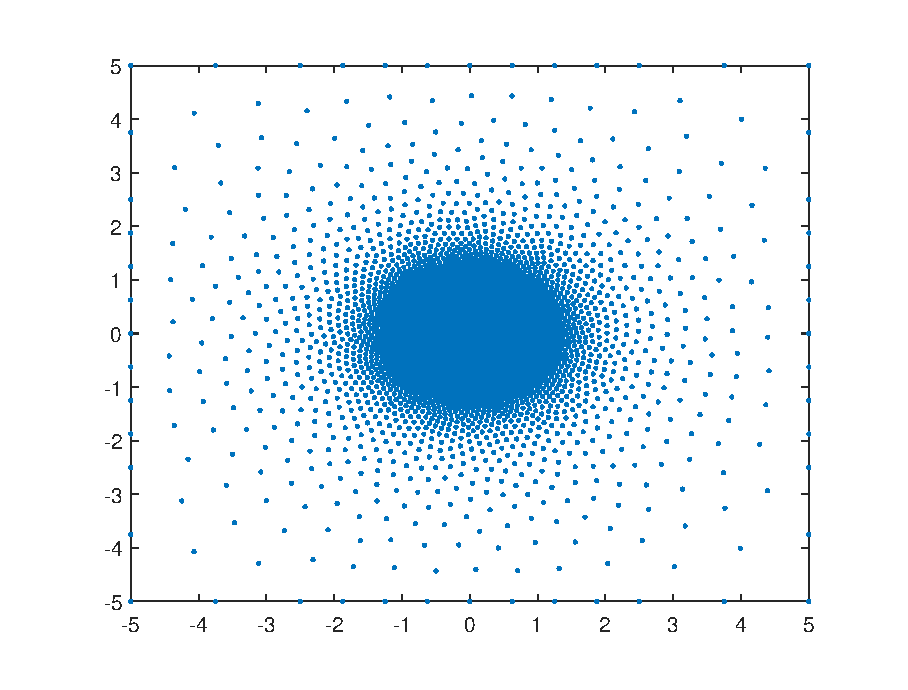
\includegraphics[width=160pt,height=120pt]{./pictures/ch2_gpu.eps}
        \end{minipage}
    }
    \subfloat[6243 bubbles generated by GPU]{
        \begin{minipage}[top]{160pt}
            \centering
            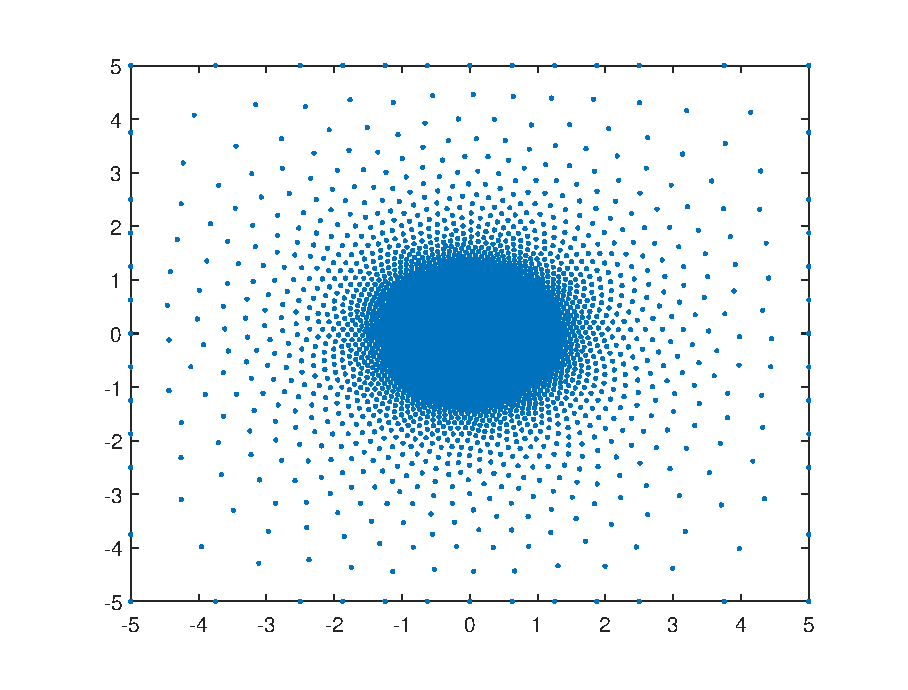
\includegraphics[width=160pt,height=120pt]{./pictures/ch2_cpu.eps}
        \end{minipage}
    }
    \caption{Comparison between two different ways}
\end{figure}



\subsection{Ideal spacing function}
In bubble grids method, ideal spacing function is used to describe the
distribution of bubbles.
Because bubbles might be placed in everywhere of the bounded area,
ideal spacing function must be a continuous function\cite{12,13}.
However, the numerical method of this paper can't provide a continuous
ideal spacing function but by interpolation.
Considering of the scattered nodes, radial basis function
interpolation was used in this paper,
which is a existing function in module scipy of python.
By inputting the nodes and values on nodes,
we can get a continuous ideal spacing function.

The initial grids of every numerical example are regular.
As the probability density $p({\bf x})$ changing, the grid
will be regenerated by bubble grid method. In order to
improve the accuracy, nodes should gather where probability
density is high. Therefore, the ideal spacing function
we choose is (\ref{ISF}).
\begin{equation}
    \label{ISF}
    d({\bf x}) = \left\{ \begin{aligned}
        & b - kh,            & p^c({\bf x}) > h \\
        & b - kp^c({\bf x}), & p^c({\bf x}) < h \\
    \end{aligned} \right.
\end{equation}
Here, $p^c({\bf x})$ is the continuous probability density
function after interpolation. $b,k$ and $h$ are some
experienced parameters. Because the probability density
function we get by numerical method is discreted, we
get $p^c({\bf x})$ by interpolating $p({\bf x})$
using radial basic function method.

% \subsection{Some changes on solving ODE equations}
% When the bubbles simulate the

\section{Adaptive path integration method on dynamic bubble grids}
The derivation of the API method is straightforward. The idea of original path integration
is to compute the long-term transition of probability distribution in small steps and the compu-
tation can be performed in a reduced finite range, $\Omega_r$, in the state space $\Omega$.
This finite range is so determined that the probability values outside the range is sufficiently
low that its effect can be neglected. We can express a typical evolution of a probability
density $p(x, t)$ from time $t_{n-1}$ to $t_n$ as follows:
\begin{equation}\label{p1}
    p^{n}({\bf x}):=p({\bf x},t_n)=\int\limits_{\Omega_r}q\left({\bf
    x},t_n|{\bf \widetilde{x}},t_{n-1}\right)p({\bf
    \widetilde{x}},t_{n-1}){\rm d}{\bf \widetilde{x}}.
\end{equation}

In order to illustrate how dynamic grids work, let $\{{\bf x}_s^{(n)}\}_{s=1}^{N_n}$ represents the grid nodes on $t_n$.
After the grid changes from $\{{\bf x}_s^{(n-1)}\}_{s=1}^{N_{n-1}}$  to $\{{\bf x}_s^{(n)}\}_{s=1}^{N_n}$ ,
$p^{n}({{\bf x}^{(n)}})$ should be interpolated from $p^{n}({{\bf x}^{(n-1)}})$ and $m_{ij}({{\bf x}^{(n)},t_n})$
should be interpolated from $m_{ij}({{\bf x}^{(n-1)},t_n})$. After that, ${\bf x}$ and ${\bf \widetilde{x}}$ in (\ref{p1})
are equivalent.
$q({\bf x},t_n|{\bf \widetilde{x}},t_{n-1})$ can be calculated by  $m_{ij}({{\bf x}^{(n)},t_n})$.
% Here, \(\{x_s^{n}\}_{s=1}^{N}\) can be generated by $p^{n}({\bf x})$ using bubble grid method or some other methods.

The numerical integration can be expressed as: (should be modified)
\begin{equation}\label{mpi1}
    p^{n}({\bf
    x}_j)=\sum\limits_{s=1}^{N_n}\left[S_{\Omega_s}q\left({\bf
    x}_j,t_n|{\bf \widetilde{x}}_{s},t_{n-1}\right)p^{n-1}({\bf
    \widetilde{x}}_{s})\right]+\mathcal{O}(h^2),\ (j=1,\cdots,N).
\end{equation}
Here $S_{\Omega_s}$ is the area of $\Omega_s$. Nodes of grid  $\{{\bf x}_s^{(0)}\}_{s=1}^{N_0}$ 
might be scattered.
Therefore, we use delaunay triangulation and  $\{\Omega_s\}_{s=1}^{N}$ is the voronoi diagram of
$\{{\bf x}_s\}_{s=1}^{N}$.

The corresponding algorithm is given as follows:
\begin{enumerate}
    \item Generate the first grid  $\{{\bf x}_s^{(0)}\}_{s=1}^{N_0}$ by initial $p^{0}({{\bf x}})$. 
    $p^{0}({{\bf x}})$ is a continuous function and $p^{0}({\bf x}^{(0)})$ can be acquired directly.
    \item Use path integration method to calculate $p^{n}({\bf x}^{(n-1)})$ on $\{{\bf x}_s^{(n-1)}\}_{s=1}^{N_{n-1}}$.
    \item Based on the improved bubble grid method with GPU, genarate grid $\{{\bf x}_s^{(n)}\}_{s=1}^{N_{n}}$ to replace $\{{\bf x}_s^{(n-1)}\}_{s=1}^{N_{n-1}}$.
    \item Interpolate $m_{ij}({{\bf x}^{(n)},t_n})$ and $p^{n}({\bf x}^{(n)})$ and turn to step 2 until it is enough. 
\end{enumerate}

\section{Numerical examples}
In this section, two specific 2D nonlinear dynamical systems, 
Duffing oscillator subjected to white noise excitation and
Duffing oscillator subjected to harmonic and stochastic
excitations(both sinusoidal and white noise excitations),
are solved on the rectangular grids via the numerical path
integration method. Duffing oscillator subjected to white
noise has exact solution which can be used to compare with
the numerical result to verify the correctness of the method
proposed in this paper. The 2D initial Gaussian distributions
are assumed as
\begin{equation}
    \label{IG2}
    q({\bf x},0)=\frac{1}{2\pi|{\bf
    B}|^{1/2}}\exp\left\{-\frac{1}{2}(\bf x-a_0)^T{\bf B}^{-1}(\bf
    x-a_0)\right\},
\end{equation}
where ${\bf x}=(x,y)^T\in\Omega_r$, $a_0=(\mu_1,\mu_2)^T$ and
${\bf B}=\left[
\begin{array}{cc}
s_1^2&s_1s_2r_{12}\\
s_1s_2r_{12}&s_2^2\\
\end{array}\right]$.
\subsection{Duffing oscillator subjected to white noise exitation}
Firstly, we consider a Duffing oscillator subjected to white noise excitation,
governed by the following equation of motion:
\begin{equation}
    \label{first_example}
    \ddot x + \eta \dot x + \alpha x + \beta {x^3} = \sigma \xi (t)
\end{equation}
where $\xi(t)$ is a Gaussian white noise with zero mean and
unit intensity. Its exact stationary solution of probability density
can be calculated when 
    $ \alpha \neq 0,\beta  > 0 $
and the exact solution can be expressed as follows:
\begin{equation}
    \label{real_result}
    P^e(x,y) = C\exp \{  - \frac{\eta }{{{\sigma ^2}}}[\alpha {x^2} + \frac{\beta }{2}{x^4} + {y^2}]\}
\end{equation}
The normalization parameter $C$ satisfies condition
$\int\limits_{ - \infty }^\infty  {\int\limits_{ - \infty }^\infty  {f(x,y)dxdy = 1} }$.

As for numerical results for (\ref{first_example}), the equations for the first- and 
second-order moments on the basis of Gaussian closure are given by
\begin{equation}
    \label{first_DM}
\left\{
\begin{array}{l}
\dot{m}_{10}=m_{01},\\
\dot{m}_{01}=-\eta m_{01}-\alpha m_{10}-3\beta m_{10}m_{20}+2\beta
m_{10}^3,\\
\dot{m}_{11}=m_{02}-\eta m_{11}-\alpha m_{20}-3\beta
m_{20}^2+2\beta
m_{10}^4,\\
\dot{m}_{20}=2m_{11},\\
\dot{m}_{02}=-2\eta m_{02}-2\alpha m_{11}-6\beta
m_{20}m_{11}+4\beta m_{10}^3 m_{01}
+\sigma^2,\\
\end{array}\right.
\end{equation}
where $m_{ij}=E[x^i,y^j]=E[x^i,\dot{x}^j]$.The Eq. (\ref{first_DM}) are some
time-dependent ODEs, which can be solved by any stable ODE
solver which retains the spatial accuracy of the method. In the
numerical examples below, we have used the fourth-order
natural continuous extensions of Runge-Kutta (NCERK) method.

Therefore, the 2D transitional Gaussian distributions are derived
as
\begin{equation}\label{TG2}
q\left({\bf x},t_n|{\bf
\widetilde{x}},t_{n-1}\right)=\frac{1}{2\pi|{\bf B}({\bf
\widetilde{x}},t_n)|^{1/2}}\exp\left\{-\frac{1}{2}\left[\bf
x-a({\bf \widetilde{x}},t_n)\right]^T{\bf B}({\bf
\widetilde{x}},t_n)^{-1}\left[\bf x-a({\bf
\widetilde{x}},t_n)\right]\right\},
\end{equation}
where ${\bf x}=(x,y)^T$, ${\bf
\widetilde{x}}=(\widetilde{x},\widetilde{y})^T$ and
$a_0=[m_{10}({\bf \widetilde{x}},t_n),m_{01}({\bf
\widetilde{x}},t_n)]^T$ and
\begin{displaymath}
{\bf B}({\bf \widetilde{x}},t_n)=\left[
\begin{array}{cc}
m_{20}({\bf \widetilde{x}},t_n)-[m_{10}({\bf \widetilde{x}},t_n)]^2 & m_{11}({\bf \widetilde{x}},t_n)-m_{10}({\bf \widetilde{x}},t_n)m_{01}({\bf \widetilde{x}},t_n)\\
m_{11}({\bf \widetilde{x}},t_n)-m_{10}({\bf \widetilde{x}},t_n)m_{01}({\bf \widetilde{x}},t_n) & m_{02}({\bf \widetilde{x}},t_n)-[m_{01}({\bf \widetilde{x}},t_n)]^2\\
\end{array}\right].
\end{displaymath}
% 原方程有稳态解,因此随便给它一个初值,它都会随着时间变化收敛到精确解。
% 这一段话要写转移方程和转移矩阵。
% 还要解释图中变量的含义

In sections 4.1.1-4.1.2, we calculate the numerical results
and exact solutions of Eq. (\ref{first_example}) respectively for different 
parameters.
%for every given parameters $\alpha, \beta, \eta, \sigma$ and obtain the numerical errors.

\subsubsection{First Example}
%{\(\alpha = -1.0,\;\beta = 0.2,\;\eta = 0.2,\;\sigma^2 = 0.5,\;C = 0.0297\)}
Hence, we choose the following system and
excitation parameters for the first example: $\alpha=-1.0$, $\beta=0.2$, $\eta=0.2$,
$\omega=1.2$ and $\sigma^2=0.5$. Then parameter $C$ in (\ref{real_result}) which can be calculated
is 0.0297. Knowing the probability density ranges from $0$ to $0.1$,
the ideal spacing function can be chosen as
\[d({\bf x}) = \left\{ \begin{aligned}
    &0.05,                & p^c({\bf x}) > 0.1 \\
    &0.15 - p^c({\bf x}), & p^c({\bf x}) < 0.1 \\
\end{aligned} \right.\]
%% 贴图
\begin{figure}[htbp]
    \centering
    \subfloat[numerical result]{
        \label{fig:subfig:1a}
        \begin{minipage}[top]{200pt}
            \centering
            \includegraphics[width=160pt,height=120pt]{./pictures/ex1_2.jpg}
        \end{minipage}
    }
    \subfloat[bubble grids depends on \(P(x,y)\)]{
        \label{fig:subfig:1b}
        \begin{minipage}[top]{200pt}
            \centering
            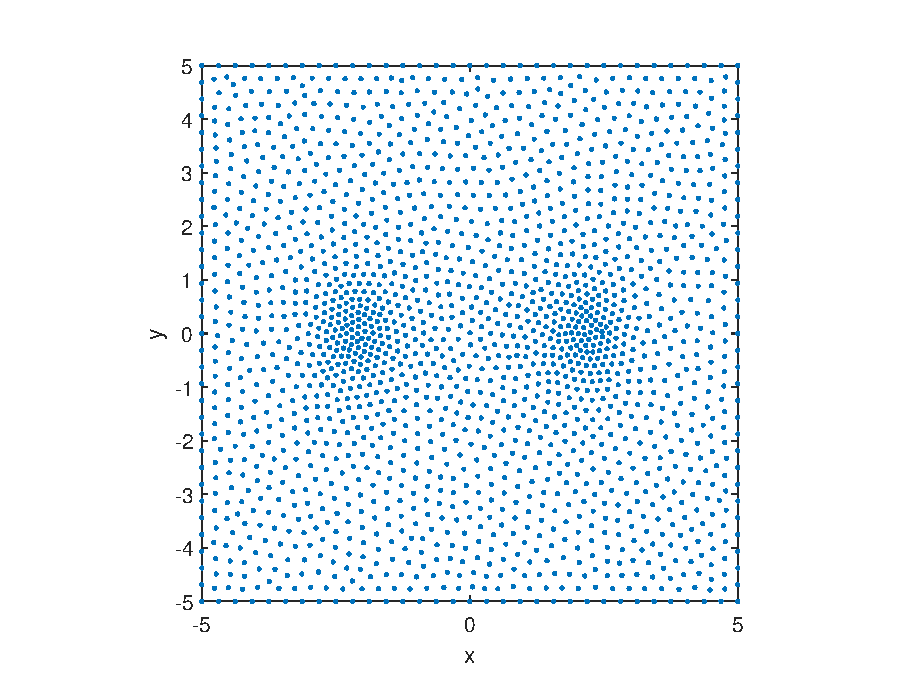
\includegraphics[width=160pt,height=120pt]{./pictures/ex1_1.eps}
        \end{minipage}
    }\\
    \subfloat[comparision of marginal probability]{
        \label{fig:subfig:1c}
        \begin{minipage}[top]{200pt}
            \centering
            \includegraphics[width=160pt,height=120pt]{./pictures/ex1_3.jpg}
        \end{minipage}
    }
    \subfloat[relation between errors and time]{
        \label{fig:subfig:1d}
        \begin{minipage}[top]{200pt}
            \centering
            \includegraphics[width=160pt,height=120pt]{./pictures/ex1_4.jpg}
        \end{minipage}
    }
    \caption{First example}
    \label{fig:1}
\end{figure}
\begin{figure}[htbp]
    \centering
    \subfloat[numerical result]{
        \label{fig:subfig:2a}
        \begin{minipage}[top]{160pt}
            \centering
            \includegraphics[width=160pt,height=120pt]{./pictures/ex2_2.jpg}
        \end{minipage}
    }
    \subfloat[bubble grids depends on \(P(x,y)\)]{
        \label{fig:subfig:2b}
        \begin{minipage}[top]{160pt}
            \centering
            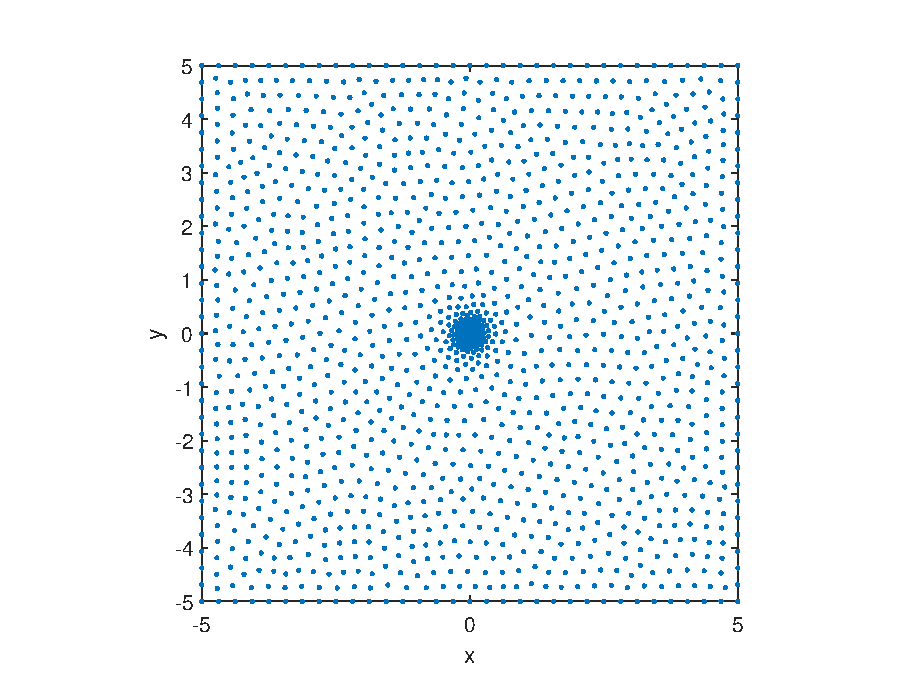
\includegraphics[width=160pt,height=120pt]{./pictures/ex2_1.eps}
        \end{minipage}
    }\\
    \subfloat[comparision of marginal probability]{
        \label{fig:subfig:2c}
        \begin{minipage}[top]{160pt}
            \centering
            \includegraphics[width=160pt,height=120pt]{./pictures/ex2_3.jpg}
        \end{minipage}
    }
    \subfloat[relation between errors and time]{
        \label{fig:subfig:2d}
        \begin{minipage}[top]{160pt}
            \centering
            \includegraphics[width=160pt,height=120pt]{./pictures/ex2_4.jpg}
        \end{minipage}
    }
    \caption{Second example}
    \label{fig:2}
\end{figure}



At first, there are 2500 regular nodes in computation domain $[-5,5] \times [-5,5]$.
Then the number of nodes gradually changes to 1822 showed in Fig.\;\ref{fig:subfig:1b}.

The time step $\triangle t$ is $T/4$
with $T=2\pi/\omega$ and the parameters of the initial Gaussian
distribution are $\mu_1=\mu_2=-1.0$, $s_1^2=s_2^2=0.1$ and
$r_{12}=0.01$. For the first example,
we calculate the computational results until $t=30T(\approx 157.07)$.
Fig.\;\ref{fig:subfig:1a} shows the numerical result.
Fig.\;\ref{fig:subfig:1b} shows the nodes generated by adaptive bubble grids method.
$P(\bf x)$ denotes marginal probability density
$\int\limits_{ - \infty }^\infty {P(x,y)dy}$ and Fig.\;\ref{fig:subfig:1c}
shows the error of $P(\bf x)$.
Fig.\;\ref{fig:subfig:1d} shows how the maximum 
absolute error declines as time goes by.

% I choose the listed parameters:\;\(\omega = 1.2 \),\;\(T = 2 \pi / \omega \),\;\(\Delta t = T / 4\) .
% I calculate example 1 , 3 and 4 until \(30 T \) when \(t \approx 157.07\) . 
% I caluculate example 2 until \(90 T\) when \(t \approx 471.24\) .

%% 绘制表格
\subsubsection{Second Example}
we choose another group of excitation parameters:
$\alpha=1.0$, $\beta=0.8$, $\eta=0.6$ and $\sigma^2=0.3$
while the rest conditions are the same with the first example. Here, the ideal
spacing function can be chosen as
\[d({\bf x}) = \left\{ \begin{aligned}
    &0.025,                     & p^c({\bf x}) > 0.7 \\
    &0.165 - 0.2p^c({\bf x}),   & p^c({\bf x}) < 0.7 \\
\end{aligned} \right.\]

For the second example,
we calculate the computational results until $t=30T(\approx 157.07)$.
Fig.\;\ref{fig:subfig:2a} shows the numerical result and Fig.\;\ref{fig:subfig:2d} shows how the maximum
absolute error declines as the time goes by.


\begin{table}[htbp]
    \centering
    \caption{comparision of the maximum absolute errors}
    \begin{tabular}[c]{ccc}
        \toprule
        Examples         & ${\bf max}|P(x)-P^e(x)|$      & ${\bf max}|P(x,y)-P^e(x,y)|$ \\
        \midrule
        first example    & 0.0028      & 0.0024 \\
        %2        & 0.0389      & 0.0075 \\
        second example   & 0.0038      & 0.0177 \\
        %4        & 0.0311      & 0.0063 \\
        \bottomrule
    \end{tabular}
\end{table}





\subsection{Duffing oscillator subjected to harmonic and stochastic excitations}
\begin{figure}[htbp]
    \centering
    \subfloat[nodes at time $T/4$]{
        \label{fig:3aa}
        \begin{minipage}[top]{160pt}
            \centering
            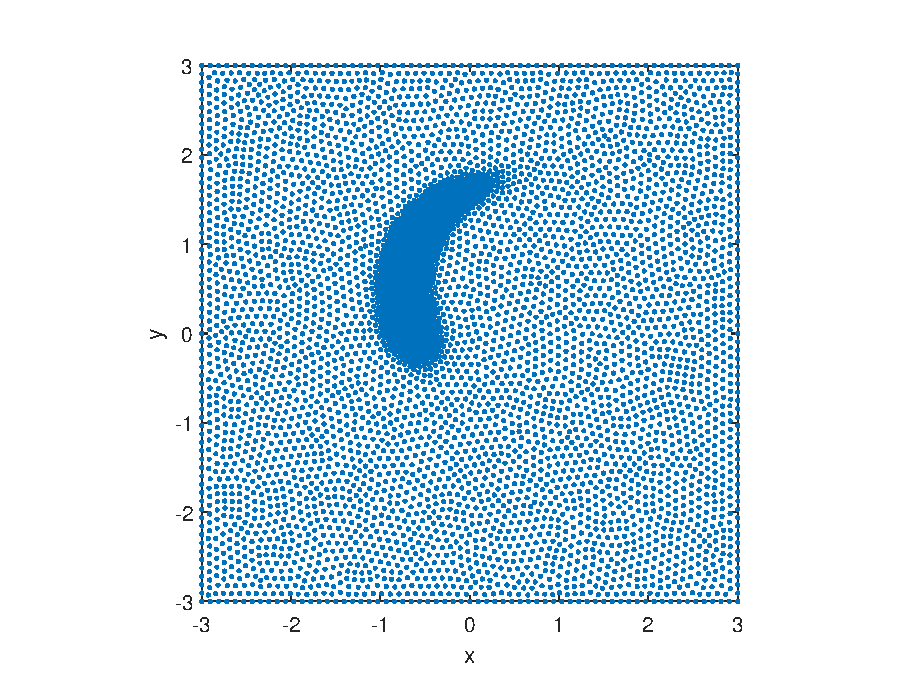
\includegraphics[width=160pt,height=120pt]{./pictures/ex3_1a.eps}
        \end{minipage}
    }
    \subfloat[surface plots at time $T/4$]{
        \label{fig:3ab}
        \begin{minipage}[top]{160pt}
            \centering
            \includegraphics[width=160pt,height=120pt]{./pictures/ex3_1b.jpg}
        \end{minipage}
    }\\
    \subfloat[nodes at time $T/2$]{
        \label{fig:3ba}
        \begin{minipage}[top]{160pt}
            \centering
            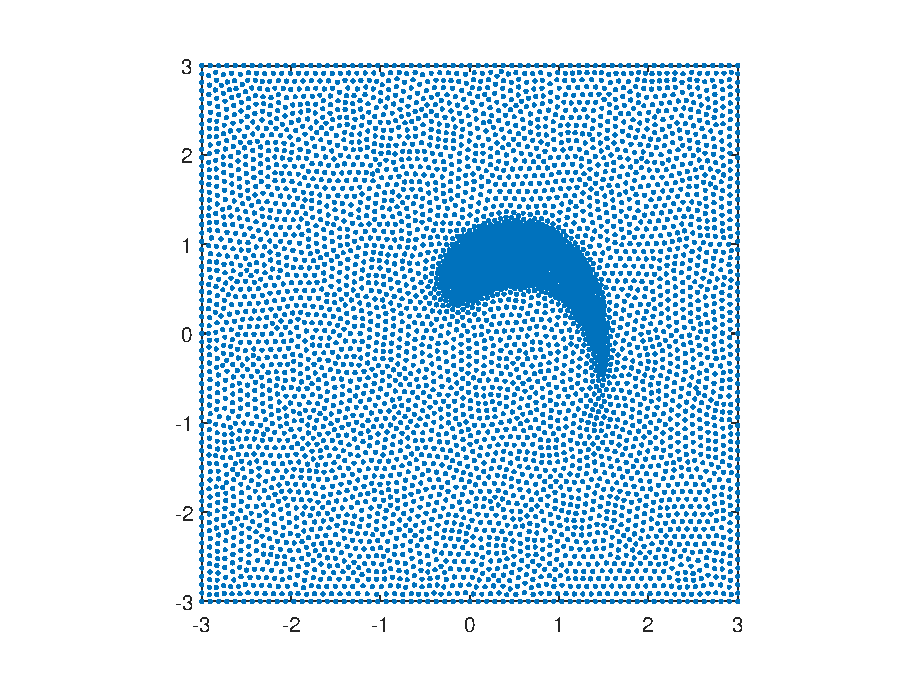
\includegraphics[width=160pt,height=120pt]{./pictures/ex3_2a.eps}
        \end{minipage}
    }
    \subfloat[surface plots at time $T/2$]{
        \label{fig:3bb}
        \begin{minipage}[top]{160pt}
            \centering
            \includegraphics[width=160pt,height=120pt]{./pictures/ex3_2b.jpg}
        \end{minipage}
    }\\
    \subfloat[nodes at time $3T/4$]{
        \label{fig:3ca}
        \begin{minipage}[top]{160pt}
            \centering
            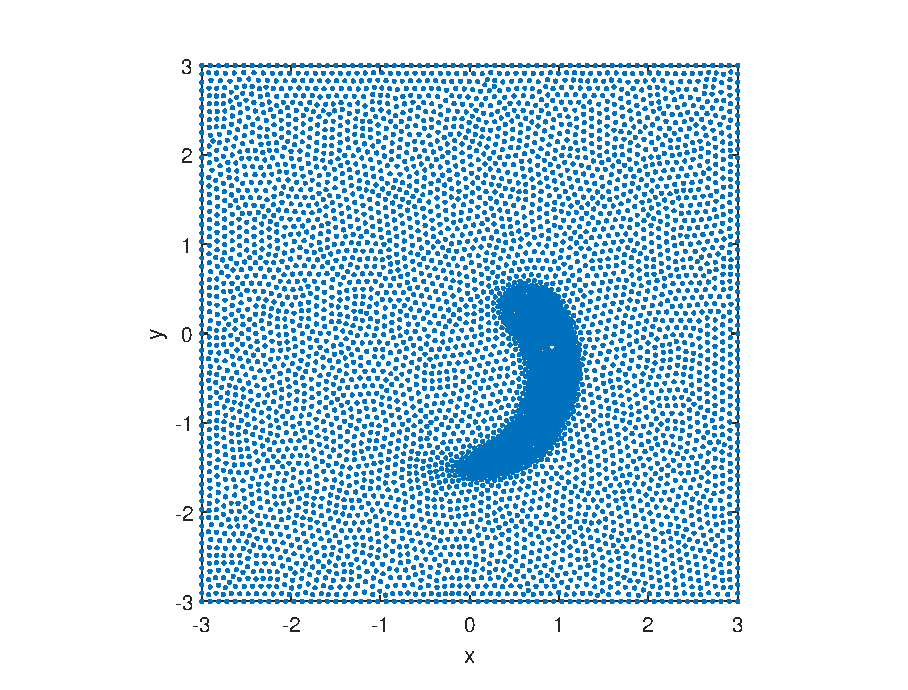
\includegraphics[width=160pt,height=120pt]{./pictures/ex3_3a.eps}
        \end{minipage}
    }
    \subfloat[surface plots at time $3T/4$]{
        \label{fig:3cb}
        \begin{minipage}[top]{160pt}
            \centering
            \includegraphics[width=160pt,height=120pt]{./pictures/ex3_3b.jpg}
        \end{minipage}
    }\\
    \subfloat[nodes at time $T$]{
        \label{fig:3da}
        \begin{minipage}[top]{160pt}
            \centering
            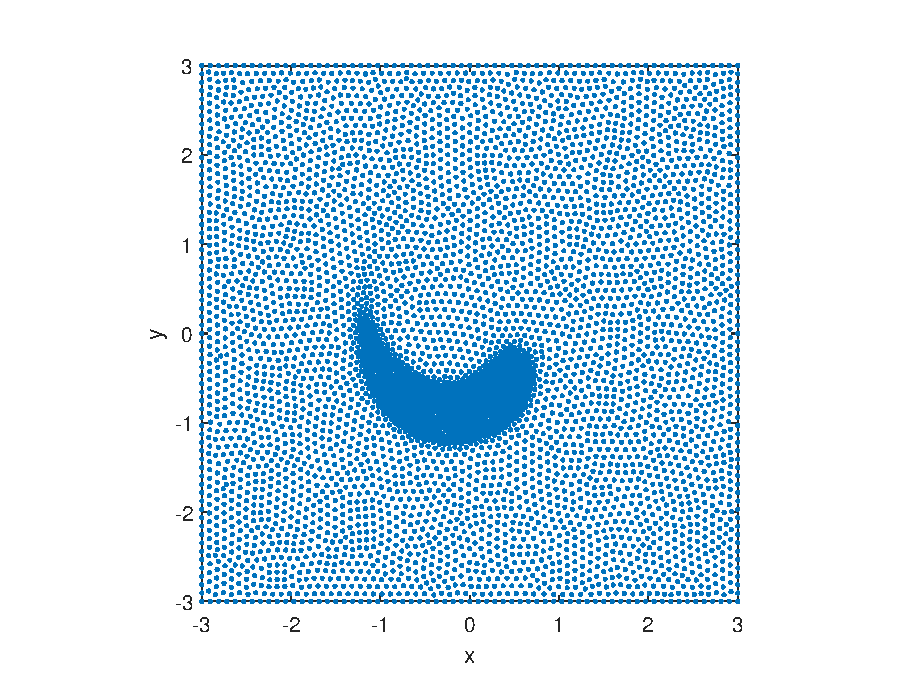
\includegraphics[width=160pt,height=120pt]{./pictures/ex3_4a.eps}
        \end{minipage}
    }
    \subfloat[surface plots at time $T$]{
        \label{fig:3db}
        \begin{minipage}[top]{160pt}
            \centering
            \includegraphics[width=160pt,height=120pt]{./pictures/ex3_4b.jpg}
        \end{minipage}
    }
    \caption{Numerical results for Duffing oscillator based on bubble grids.}
    \label{fig:3}
\end{figure}

Then we consider a Duffing oscillator subjected to both
sinusoidal and white noise excitations, governed by the following
equation of motion:
\begin{equation}\label{D}
\ddot{x}+\eta\dot{x}+\alpha x+\beta x^3=F\cos\omega
t+\sigma\xi(t),
\end{equation}
where $\xi(t)$ is a Gaussian white noise with zero mean and unit intensity.
The equations for the first- and second-order moments on the basis of
Gaussian closure are given by
\begin{equation}\label{DM}
\left\{
\begin{array}{l}
\dot{m}_{10}=m_{01},\\
\dot{m}_{01}=-\eta m_{01}-\alpha m_{10}-3\beta m_{10}m_{20}+2\beta
m_{10}^3+F\cos\omega t,\\
\dot{m}_{11}=m_{02}-\eta m_{11}-\alpha m_{20}-3\beta
m_{20}^2+2\beta
m_{10}^4+m_{10}F\cos\omega t,\\
\dot{m}_{20}=2m_{11},\\
\dot{m}_{02}=-2\eta m_{02}-2\alpha m_{11}-6\beta
m_{20}m_{11}+4\beta m_{10}^3 m_{01}
+\sigma^2+2m_{01}F\cos\omega t,\\
\end{array}\right.
\end{equation}
where $m_{ij}=E[x^i,y^j]=E[x^i,\dot{x}^j]$. Eqs.\;(\ref{DM}) are solved by the fourth-order NCERK method.

There are also 2500 regular nodes in the square computational domain,
$[-3,3]\times[-3,3]$.The ideal spacing function can be choose as
\[d({\bf x}) = \left\{ \begin{aligned}
    &0.05, & p^c({\bf x}) > 0.16\\
    &0.025 - 0.15625p^c({\bf x}), & p^c({\bf x}) < 0.16\\
\end{aligned} \right.\]
The number of nodes changes to 5327 finally.

The time step $\triangle t$ is $T/4$
with $T=2\pi/\omega$. The parameters of the initial Gaussian
distribution are $\mu_1=\mu_2=-1.0$, $s_1^2=s_2^2=0.1$ and
$r_{12}=0.01$. Here we choose the following system and
excitation parameters: $\alpha=1.0$, $\beta=0.3$, $\eta=0.1$,
$F=0.2$, $\omega=1.2$ and $\sigma^2=0.01$. 
Fig.\;\ref{fig:3} % Fig.~1 
describes the
periodic quality of the probability density, which has the good
agreement with the results in \cite{9}.


\section{Conclusions}

We present an adaptive numerical path integration method for
non-linear dynamic systems. All nodes were placed according
to the probability density values. When the probability density
changes, nodes adapt themselves to new probability density
function. Two experiments are solved successfully and some
smart dynamical behaviors of Duffing oscillator subjected to
harmonic and stochastic excitations were also described herein.

\section*{Acknowledgments}

This research was supported by the National Natural
Science Foundation of China (Grant Nos. 11871399,
11471261) and the Natural Science Foundation of
Shaanxi (Grant No. 2017JM 1005).

\begin{thebibliography}{aaa}
    \bibitem{ZWQ2017}
    W. Q. Zhu, G. Q. Cai. Introduction to Stochastic Dynamics.
    \textsl{Science Press A} 27(5) (1983) 2663-2670.
    \bibitem{GCW1986}
    C. Gardiner . Handbook of Stochastic Methods. 
    \textsl{Springer-Verlag A} (1985).
    \bibitem{1}
    M. F. Wehner, W. G. Wolfer. Numerical evaluation of path-integral solutions to Fokker-Planck equations. 
    \textsl{Physical Review A} 27(5) (1983) 2663-2670.
    \bibitem{2}
    M. F. Wehner, W. G. Wolfer. Numerical evaluation of path-integral solutions to Fokker-Planck equations II, restricted stochastic processes. 
    \textsl{Physical Review A} 28(5) (1983) 3003-3011.
    \bibitem{3}
    M. F. Wehner, W. G. Wolfer. Numerical evaluation of path-integral solutions to Fokker-Planck equations III, time and functionally dependent coefficients. 
    \textsl{Physical Review A} 35(4) (1987) 1795-1801.
    \bibitem{4}
    A. Naess, V. Moe. Efficient path integration methods for nonlinear dynamic systems. 
    \textsl{Probabilistic Engineering Mechanics} 15 (2000) 221-231.
    \bibitem{5}
    J. S. Yu, G. Q. Cai, Y. K. Lin. A new path procedure based on Gauss-Legendre scheme. 
    \textsl{International Journal of Non-Linear Mechanics} 32(4) (1997) 759-768.
    \bibitem{6} J. S. Yu, Y. K. Lin. Numerical path integration of a non-homogeneous Markov process. 
    \textsl{International Journal of Non-Linear Mechanics} 39 (2004) 1493-1500.
    \bibitem{7} P. Kumar, S. Narayanan, Numerical solution of multidimensional Fokker–Planck equation for nonlinear stochastic dynamical systems.
    \textsl{Advances in Vibration Engineering} 8(2) (2009) 153–163.
    \bibitem{8} P. Kumar, S. Narayanan, Modified path integral solution of Fokker–Planck equation: response and bifurcation of nonlinear systems.
    \textsl{ASME Journal of Computational and Nonlinear Dynamics} 5(1) (2010) 011004.
    \bibitem{9} W. X. Xie, W. Xu, L. Cai, Numerical meshfree path integration method for non-linear dynamic systems.
    \textsl{Applied Mathematics and Computation} 197 (2008) 426-434.
    
    \bibitem{10} L. Cai, Y. Nie, W. X. Xie, W. Zhang. Numerical path integration method based on bubble grids for nonlinear dynamical systems.
    \textsl{Applied Mathematical Modelling} 37(3) (2013) 1490-1501.
    \bibitem{11} K. Shimada and D. Gossard. Bubble mesh: automated triangular meshing of non-manifold geometry by spherepacking.
    \textsl{In Proceedings of the third ACM symposium on Solid modeling and applications} (1995) 409–419.
    \bibitem{12} Y. Liu, Y. Nie, W. Zhang, and L. Wang. Node placement method by bubble simulation and its application.
    \textsl{Computer Modeling in Engineering \& Sciences} 55(1) (2010) 89–109.
    \bibitem{13} W. Chen, Y. Nie, W. Zhang, and L. Wang. A fast local mesh generation method about high-quality node set.
    \textsl{Jisuan Lixue Xuebao/Chinese Journal of Computational Mechanics} 29(5) (2012) 704–709.
    \bibitem{14} W. Zhang, Y. Nie, and Y. Gu. Adaptive finite element analysis of elliptic problems based on bubble-type local mesh generation.
    \textsl{Journal of Computational and Applied Mathematics} 280 (2015) 42–58.
    \bibitem{15} W. Zhang, Y. Nie, L. Cai, and N. Qi. An adaptive discretization of incompressible flow using node-based local meshes.
    \textsl{Computer Modeling in Engineering \& Sciences} 102(1) (2014) 55-82.
    \bibitem{16} F. Wang, Y. Nie, W. Zhang, et al. NPBS-based adaptive finite element method for static electromagnetic problems[J]. 
    \textsl{Journal of Electromagnetic Waves and Applications} 30(15) (2016) 19.
    \bibitem{17} W. Guo, Y. Nie, W. Zhang. Parallel adaptive mesh refinement method based on bubble-type local mesh generation[J]. 
    \textsl{Journal of Parallel \& Distributed Computing} (2018) 117.

\end{thebibliography}

\end{document}